% !TEX root = ../master.tex
\chapter{Fundamentals}
\label{chap:fund}

TODO

\section{Big Data, \acl{BIA} and \acl{BDA}}

Chen et.~al characterize \ac{BIA} as \blockcquote[p.~1166]{chen2012business}{the techniques, technologies, systems, practices, methodologies, and applications that analyze critical business data to help an enterprise better understand its business and market and make timely business decisions}. Its goals and methodology closely resembles that of the emerging field of \ac{BDA} \autocite[][p.~1166]{chen2012business}. 
According to Chen et.~al and their involvement in the \ac{BIA} space from the end of the last century to the 2010s three major evolutionary phases of the sector may be differentiated, with \ac{BDA} characterizing the evolution in the last stage \autocite[][p.~1168 \psqq]{chen2012business}. In order to provide an overview regarding the development of the context area, the different stages will be looked at and briefly characterized hereafter.

In the first evolutionary phase, identified as \textbf{\ac{BIA} 1.0}, the desire for the storage and analysis of business data emerged. Companies started to utilize already existing \acp{RDBMS} to store mostly structured data collected from various legacy systems such as mainframes. This phase includes the usage of statistical methods to generate and validate new hypotheses regarding stored information, widely known as \ac{DM}. In this regard the main emphasis of \ac{BIA} departments was to design, deploy and maintain data warehouses with optimized \ac{ETL} cycles in order to regularly feed new data into the system using batch processing. The stored information may then be analyzed using \ac{OLAP} systems and are usually visualized with dashboards and graphs to allow a better insight for the end-users.
Most of the currently deployed analytic platforms, including standard software by common software vendors such as Microsoft or Oracle, are based on the technologies developed in the \ac{BIA} 1.0 phase. Although these developments already started in the 1970s and accelerated in the 1980, there is still ongoing research and active feature implementation until today. \autocite[Cmp.][p.~1166 \psq]{chen2012business}

As the Web 2.0 became popular in the early 2000s, an unknown variety of data sources emerged as well. The goal of the \textbf{\ac{BIA} 2.0} ignited by these events is to harvest the new opportunities for analytical processing created by this additional data. The collection of statistics on an individual customer basis allowed to generate a better understanding of customer's needs and thus offer tailored goods and services to a company's clients.
Moreover, the invention of social media platforms led to a massive influx of publicly available user-generated content. The analysis of such unstructured data posed the main challenge to traditional applications, focused on structured data with well-defined schemes. Although some techniques and opportunities addressed by \ac{BIA} 2.0 have been incorporated into commercial offerings, there still exists a large room for future growth. Especially the techniques of text mining, social network and spatial-temporal analysis are still under active academic investigation. \autocite[Cmp.][p.~1167 \psq]{chen2012business}

Finally, the most interesting phase in the context of \ac{BDA} is that of \textbf{\ac{BIA} 3.0}. Sparked by an exponentially increasing volume of data due to mobile and \ac{IoT} devices, that \enquote{traditional} systems are not capable of dealing with, this term represents a new research area currently in development. The enormous desire of enterprises to gain meaningful insight from the \blockcquote[p.~1168]{chen2012business}{massive, location-aware, person-centered and context-relevant data} in a so-called Web 3.0 environment is leading both IT vendors and academia to develop tailor-fit solutions. However, as of today,  no comprehensive standard software is commercially available yet, and neither are academic courses that educate the workforce of tomorrow. \autocite[Cmp.][p.~1168]{chen2012business}

Rajasekar et. al. establishes a understanding on the definitions and tools of \ac{BDA}, enriched by offering a comparison with traditional \acp{DBMS} regarding size and type of the underlying input data \autocite[Cmp.][p.~80]{rajasekar2015survey}. Accordingly, \ac{BDA} is concerned with the analysis of the \enquote{massive amount of un-, semi- and structured data too large to be handled by traditional DBMS}. The property of being too large is therefore strongly dependent on the precise \ac{DBMS} in use \autocite[Cmp.][p.~80]{rajasekar2015survey}, and the threshold level might change in the future as technological advancements enable legacy software to process larger data quicker. However, additional processing power created by technological advancements is unlikely to keep up with the exponential growth of incoming data. \autocite[Cmp.][p.~80\psq]{rajasekar2015survey}

\begin{table}[hbt]
	\begin{tabular}{l|ll}
	  \textbf{Characteristic} & \textbf{Traditional \acp{RDBMS}} & \textbf{\acf{BDA}} \\[0.5em]
	  \hline
	  Data Size & Gigabytes & Petabytes \\
	  Access Type & Interactive and Batch & Batch only \\
	  Update Frequency & Continuously Read and Write & Write once, Read continuously \\
	  Schema Type & Static & Dynamic \\
	  Data Integrity & High & Low \\
	  Scaling Behavior & Nonlinear & Linear \\
	\end{tabular}
	\caption{Comparison of typical \acl{RDBMS} and \acl{BDA} properties. Reprinted with adaptions from \cite[p.~80]{rajasekar2015survey}}
	\label{fig-dbms-vs-bda}
\end{table}


In order to compare the most important properties of traditional \acp{RDBMS} with those of
\ac{BDA} methods, i.e. \emph{MapReduce}, the authors propose a table similar to
\autoref{fig-dbms-vs-bda}. The table highlights the flexibility that is connected with \ac{BDA},
achieved by breaking up the structure of traditional system and limiting the interactive
possibilities for the prospective end users, which are traded against a much higher maximum
throughput. \autocite[Cmp.][p.~80]{rajasekar2015survey}
Furthermore, it is industrially accepted that the differences between the two data analysis
paradigms can be grouped into five dimensions, the so-called \emph{5V's}, as displayed in
\autoref{fig-5vs} \autocite[Cmp.][p.~80]{rajasekar2015survey},\autocite[Cmp.][p.~3\psq]{bhosale2014review}.

\begin{figure}[hbt]
  {\centering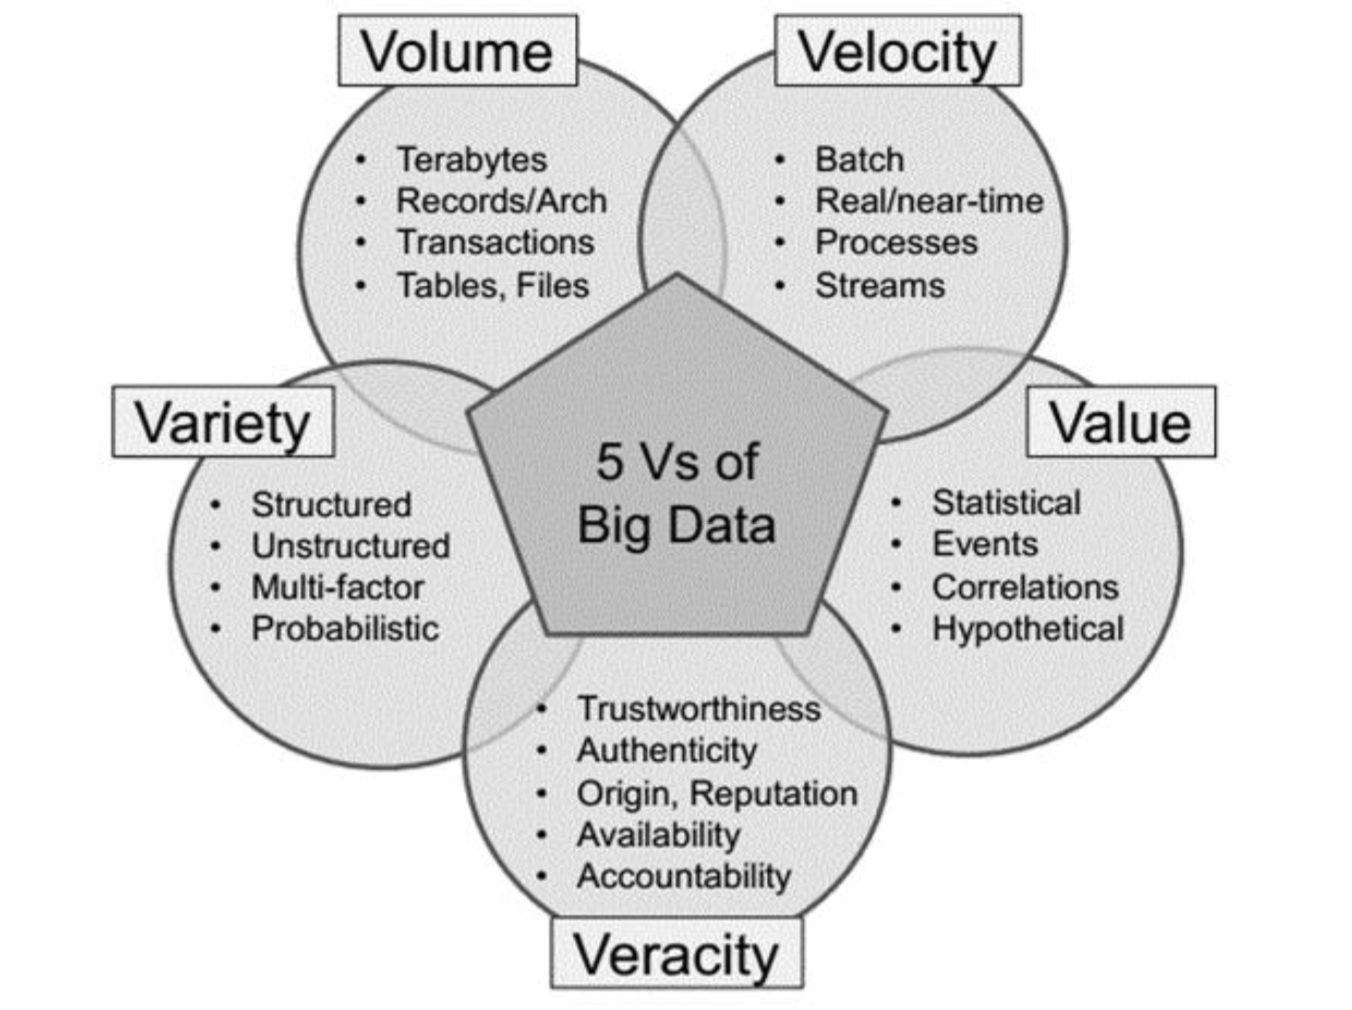
\includegraphics[width=0.75\textwidth]{{resources/big-data-parameters}.png}\par}
  \caption{The \emph{5V's} of \acl{BDA}. Reprinted from \autocite[][p.~81]{rajasekar2015survey}}
  \label{fig-5vs}
\end{figure}

As soon as data increases complexity in at least some of these dimensions, it qualifies for special treatment through \ac{BDA} systems. Although this is a common use case, as outlined in the next section, only few software solutions are available in the open market to combat these challenges. \autocite[Cmp.][p.~1182 \psqq]{chen2012business},\autocite[Cmp.][p.~80]{rajasekar2015survey}


\section{Hadoop}

TODO copy paste from jonas and phillip

\subsection{Development of Hadoop}

TODO

\subsection{Hadoop Technical Explanation}

TODO

\subsection{Hadoop at the DHBW}

TODO

\subsection{Hadoop Ecosystem}

TODO

\subsection{Map reduce shortcomings}

TODO


\section{Legal Boundaries}

When a \ac{BDA} system is actively used, it handles data in diverse forms from many sources.
Depending on the kind of data, there are different legal restriction 
to the conditions of collection, storage and processing thereof.
The main restrictive laws that are applicable for the \ac{DHBW} are the Euroean \ac{GDPR}, the German \ac{BDSG} and the \ac{HSchulDSV} Baden-Würtemberg.

The \emph{\ac{HSchulDSV} in Baden-Würtemberg}  regulates which personal data the \ac{DHBW} may collect from students and how this data may be used.
It permits the usage of personal data for \enquote{organizational or other purposes} and allows the creation of anonymized reports with it.
Personal information about students must be deleted 40 years the the student was exmatriculated. 
\autocite[][§1, §11, §12]{bw2012hcchuldsv}

The \emph{German \ac{BDSG}} regulates the general principles in data protection in Germany 
and restricts the collection, usage and storage of personal data.
In general no more data than necessary may be collected and the usage requires consent. 
The user can demand the deletion of their data.
\autocite[][§1ff., §12ff.]{bmjv2009bdsg}

The \emph{European \ac{GDPR}} is largely based
on the German regulation and introduces more control for users about their personal data.
\autocite{eu2016gdpr}
The \ac{GDPR} Portal \autocite{trunomi2018gdpr} summarizes the key changes that were introduced:
\begin{itemize}
    \item \emph{Penalties} may be imposed for organizations that breach the \ac{GDPR}.
    \item \emph{Consent} from users must be requested to collection, storage and usage of personal data. The consent may be revoked.
    \item \emph{Breach Notifications} are mandatory to inform users if data was exposed.
    \item \emph{Right to Access} for every user to their own personal data.
    \item \emph{Data Portability}, i.e. the requested data should be available to the user in a common format.
    \item \emph{Right to be Forgotten}, i.e. the right to have personal data deleted permanently upon request.
    \item \emph{Privacy by Design} for new data processing systems.
\end{itemize}

The listed laws focus on personal data, but might also be applicable to anonymized data that is derived from personal data.
Table \ref{fig-legal-data-kinds} describes which restrictions regulations apply to which type of data from which source. 
An example for the kind of data is given.

\begin{table}[hbt]
\resizebox{\textwidth}{!}{%
	\begin{tabular}{l|lll}
	  & \textbf{Internal} & \textbf{Open Source} &  \textbf{Closed Source} \\[0.5em]
	  \hline
	  \textbf{Personal} & \acs{GDPR} \& \acs{HSchulDSV} & N/A & \acs{GDPR} \& license \\
	  & e.g. student data & N/A & e.g. advertising contacts\\[0.5em]
	  \textbf{Anonymized} & possibly \acs{GDPR} \& \acs{HSchulDSV} & possibly \acs{GDPR} & possibly \acs{GDPR} \& license\\
	  & e.g. lecture statistics & e.g. social media graphs & e.g. advertising statistics\\[0.5em]
	  \textbf{Non-Personal} & unrestricted & unrestricted & restricted by license \\
	  & e.g. server monitoring & e.g. weather data & e.g. bought datasets \\
	\end{tabular}%
	}
	\caption{Kinds of data and how their use might be restricted by legislation or licenses.}
	\label{fig-legal-data-kinds}
\end{table}


When the Hadoop cluster is used at the \ac{DHBW} it might by accessed by administrative staff, lecturers and students.
However as Hadoop had not been designed with advanced user access 
and the ability to delete single records in mind,  
care must be taken to which data is stored on the Hadoop cluster.
The least restrictive solution is to use public, open source, non-personal dataset, such as academic research data, and to avoid the storage of personal student data on the cluster. 
